
\subsection{{\idletime}が一般の場合}
\label{subsec:LineDifferentTimelimit}

全点の{\idletime}が等しい場合は
どの頂点も高々1人の巡査が担当するため
単純になっていたが,
{\idletime}が一般の場合は,
頂点を複数の巡査が交代で訪問して警備する必要がある場合が存在する.
%
図\ref{tikz:multiAgentExample2}(左)の例では,
中央の{\idletime}の短い2つの頂点を
2人の巡査が交互に訪問しており,
また,全点の{\idletime}が等しい場合と異なり
各巡査の最適な運行はなんらかの区間の往復であるとは限らないことも分かる.


また,
この例では左の巡査は左端の点を{\idletime}$10$ちょうどごとに訪問しているが,
左端の点の{\idletime}から順に巡査の運行を決定することも難しい次のような例が存在する.
図\ref{tikz:multiAgentExample2}(中央)の例では
{\idletime}$8$の左端の点をあえてより短い$6$ごとに訪問することで全点を警邏できるが,
同じグラフについて,
図\ref{tikz:multiAgentExample2}(右)のように左の巡査が
左端の点の{\idletime}ぎりぎりの時間まで右の方へ動き頂点をなるべく多くの時間訪問して左端へ帰る運行を選ぶと
右の巡査がどのような動き方をしても{\idletime}を超え警備できない頂点が生まれてしまう.



\begin{figure}[h]
  \centering
  \begin{tabular}{ccc}

  \begin{minipage}{0.32\hsize}
    \centering
    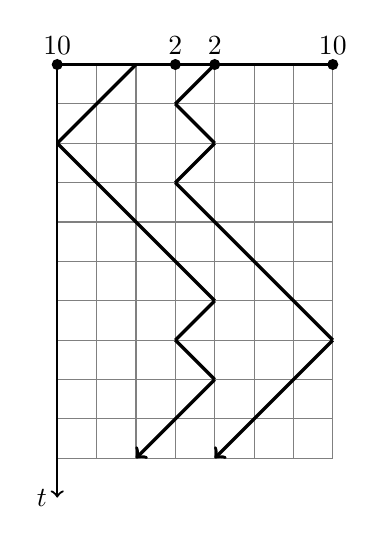
\begin{tikzpicture}
      \draw [help lines,thin,step=5mm] (0,-5.0) grid (3.5,0);
      \draw[thick] (0,0) -- (3.5,0) node [below] {};
      \draw[thick, ->] (0,0) -- (0,-5.5) node [left] {$t$};

      \fill ( 0   , 0) coordinate (c1) circle (2pt) node [above] {10};
      \fill ( 1.5 , 0) coordinate (c2) circle (2pt) node [above] {2};
      \fill ( 2.0 , 0) coordinate (c3) circle (2pt) node [above] {2};
      \fill ( 3.5 , 0) coordinate (c5) circle (2pt) node [above] {10};

      \draw[very thick,- ] ( 1.0, 0  )--(   0,-1.0);
      \draw[very thick,- ] (   0,-1.0)--( 2.0,-3.0);
      \draw[very thick,- ] ( 2.0,-3.0)--( 1.5,-3.5);
      \draw[very thick,- ] ( 1.5,-3.5)--( 2.0,-4.0);
      \draw[very thick,->] ( 2.0,-4.0)--( 1.0,-5.0);

      \draw[very thick,- ] ( 2.0, 0  )--( 1.5,-0.5);
      \draw[very thick,- ] ( 1.5,-0.5)--( 2.0,-1.0);
      \draw[very thick,- ] ( 2.0,-1.0)--( 1.5,-1.5);
      \draw[very thick,- ] ( 1.5,-1.5)--( 3.5,-3.5);
      \draw[very thick,->] ( 3.5,-3.5)--( 2.0,-5.0);
    \end{tikzpicture}
  \end{minipage}

  \begin{minipage}{0.32\hsize}
    \centering
    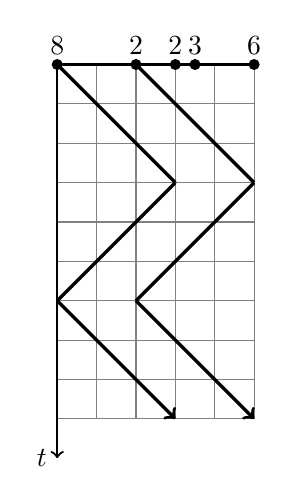
\begin{tikzpicture}
      \draw [help lines,thin,step=5mm] (0,-4.5) grid (2.5,0);
      \draw[thick] (0,0) -- (2.5,0) node [below] {};
      \draw[thick, ->] (0,0) -- (0,-5) node [left] {$t$};

      \fill ( 0   , 0) coordinate (c1) circle (2pt) node [above] {8};
      \fill ( 1   , 0) coordinate (c2) circle (2pt) node [above] {2};
      \fill ( 1.5 , 0) coordinate (c3) circle (2pt) node [above] {2};
      \fill ( 1.75, 0) coordinate (c4) circle (2pt) node [above] {3};
      \fill ( 2.5 , 0) coordinate (c5) circle (2pt) node [above] {6};

      % \draw[very thick,red,<->] (1.75,-0.75)--(1.75,-2.25);

      \draw[very thick,- ] ( 0  , 0  )--( 1.5,-1.5);
      \draw[very thick,- ] ( 1.5,-1.5)--( 0  ,-3  );
      \draw[very thick,->] ( 0  ,-3  )--( 1.5,-4.5);
      \draw[very thick,- ] ( 1  , 0  )--( 2.5,-1.5);
      \draw[very thick,- ] ( 2.5,-1.5)--( 1  ,-3  );
      \draw[very thick,->] ( 1  ,-3  )--( 2.5,-4.5);
    \end{tikzpicture}
  \end{minipage}

  \begin{minipage}{0.32\hsize}
    \centering
    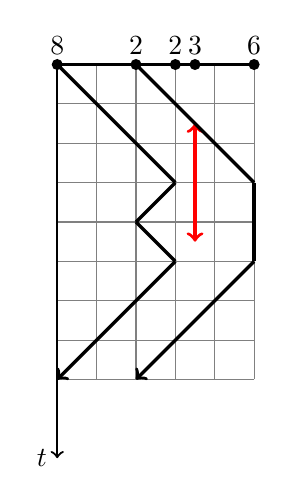
\begin{tikzpicture}
      \draw [help lines,thin,step=5mm] (0,-4) grid (2.5,0);
      \draw[thick] (0,0) -- (2.5,0) node [below] {};
      \draw[thick, ->] (0,0) -- (0,-5) node [left] {$t$};

      \fill ( 0   , 0) coordinate (c1) circle (2pt) node [above] {8};
      \fill ( 1   , 0) coordinate (c2) circle (2pt) node [above] {2};
      \fill ( 1.5 , 0) coordinate (c3) circle (2pt) node [above] {2};
      \fill ( 1.75, 0) coordinate (c4) circle (2pt) node [above] {3};
      \fill ( 2.5 , 0) coordinate (c5) circle (2pt) node [above] {6};

      \draw[very thick,red,<->] (1.75,-0.75)--(1.75,-2.25);

      \draw[very thick,- ] ( 0  , 0  )--( 1.5,-1.5);
      \draw[very thick,- ] ( 1.5,-1.5)--( 1  ,-2  );
      \draw[very thick,- ] ( 1  ,-2  )--( 1.5,-2.5);
      \draw[very thick,->] ( 1.5,-2.5)--( 0  ,-4  );

      \draw[very thick,- ] ( 1  , 0  )--( 2.5,-1.5);
      \draw[very thick,- ] ( 2.5,-1.5)--( 2.5,-2.5);
      \draw[very thick,->] ( 2.5,-2.5)--( 1  ,-4  );
    \end{tikzpicture}
  \end{minipage}

  \end{tabular}
  \caption{巡査の協力が必要な例.
    横軸を頂点の座標,縦軸を時刻として巡査の軌跡を表す.
    点の上の数値は{\idletime}を表す.
    \label{tikz:multiAgentExample2}}
\end{figure}




これらの例は,協力が発生する場合巡査の運行を個別に決定するのは難しいということを示唆している.
しかしながら,この{\idletime}が一般の場合での{\graphLine}上の{\patProb}の困難性を示すこともできなかった.
そこで,{\idletime}より短い間隔で点を訪問しうることで運行の決定を複雑になる例が存在したことを踏まえて,
1章で定義した{\timeSpecifiedPatProbDecision}を考える.






任意の運行可能集合$X$に対して,
{\graphLine}上の巡査の運行$a$であって,
$X$のすべての元$(t, x)$に対して$a(t) = x$を満たすものが存在することは簡単に示すことができる.
これにより,
グラフが{\graphLine}の場合の{\timeSpecifiedPatProbDecision}は次のようにも記述できる.

\begin{defi}
  $S \subset \Zset \times \Nset$とする.
  任意の$(t_1, x_1), (t_2, x_2) \in S$が
  $\abs{x_1 - x_2} \leq \abs{t_1 - t_2}$
  を満たすとき,$S$は運行可能であるという.
  また,分割$\{ P_1, \ldots, P_l \}$が運行可能であるとは,
  各$P_1, \ldots, P_l$が運行可能集合となることである.
\end{defi}

\begin{timeSpecifiedProblemOnLine}
  正の整数$m$(巡査の人数を表す)
  と自然数の組$(q_i, r_i, x_i)_{ i \in \{ 1, \ldots, n \} }$が与えられる.
  集合
  $\{ (q_i k + r_i, x_i) \mid i \in \{1, \ldots, n\}, k \in \Zset \}$
  を$m$個以下の運行可能集合に分割できるか判定せよ.
\end{timeSpecifiedProblemOnLine}


この問題では,
$X := \{ (q_i k + r_i, x_i) \mid i \in \{1, \ldots, n\}, k \in \Zset \}$
という無限集合の分割が可能か判定しなければならないが,
実際には$X$の点は時刻(組$(t, x) \in X$の第1要素)について周期的であるため,
1周期分の有限部分集合を以下に定義する「繰り返し運行可能な」集合に分割できるかどうかさえ
判定すればよい.


\begin{defi}
  $T$を正の整数,$S \subset \Zset \times \Nset$を有限集合とする.
  任意の$(t_1, x_1), (t_2, x_2) \in S$が
  $\abs{x_1 - x_2} \leq \abs{t_1 - t_2}$
  かつ
  $\abs{x_1 - x_2} \leq \abs{T + t_1 - t_2}$
  を満たすとき,$S$は周期$T$で繰り返し運行可能であるという.
  また,分割$\{ P_1, \ldots, P_l \}$が周期$T$で繰り返し運行可能であるとは,
  各$P_1, \ldots, P_l$が周期$T$で繰り返し運行可能となることである.
\end{defi}



以下では,集合$S$に対して
$S[a:b] := \{ (t, x) \in S \mid a \leq t < b \}$
と記号を定義する.
また,$T := lcm(q_1, \ldots, q_n)$とする(
$q_1, \ldots, q_n$は{\timeSpecifiedPatProbOnLine}の入力のもの).


$X$全体を$m$個の運行可能集合に分割できるとき,
部分集合$X[-T: 2T]$を
後で述べる{\setPartitionAlgorithm}で分割すると,
大きさ$m$以下の分割 $\mathcal{P} = \{ P_1, \ldots, P_l \}$ が得られる.
%
一方,
$X[-T: 2T]$を
{\setPartitionAlgorithm}で分割した結果が
$\{ P_1, \ldots, P_l \}$となるとき,
$\{ P_1[0:T], \ldots, P_l[0:T] \}$は$X[0:T]$に対する
分割でありかつ周期$T$で繰り返し運行可能となる
\red{←どう説明?}
.
よって,
$X[kT:(k + 1)T]$を$X[0:T]$と同様に分割したものを
$C_k := \{ C_{k1}, \ldots, C_{kl} \}$とすると,
$A_i := \bigcup_{k \in \Zset} C_{ki}$として
$\mathcal{A} := \{ A_1, \ldots, A_l \}$は
$X$の運行可能分割となる.


以上から,$X$を$m$個の運行可能集合へ分割できるかどうかは,
$X[-T:2T]$を{\setPartitionAlgorithm}により分割した結果$\mathcal{P}$が
$\card{\mathcal{P}} \leq m$を満たすかどうかで判定できる.



\begin{greedyAlgorithmForTimeSpecifiedProblemOnLine}
  入力を$S$とする.
  初期値を$\mathcal{P} = \{\}$, $S' = S$とし,
  $S' \neq \emptyset$である限り1.から3.を繰り返す.
  \begin{enumerate}
    \item $P \gets
      \{ (t, x) \in S' \mid x - \beta \leq \abs{t - \alpha} \}$
    \item $\mathcal{P} \gets \mathcal{P} \cup \{ P \}$.
    \item $S' \gets S' \setminus P$, 
  \end{enumerate}
  $\mathcal{P}$を出力する.
  $\blacksquare$
\end{greedyAlgorithmForTimeSpecifiedProblemOnLine}

{\setPartitionAlgorithm}は,
有限集合$S$を入力として,
$S$の最小の運行可能分割であって「順序保存」なものを出力する.
運行可能分割が順序保存であるとは,
その分割から順序保存運行が生成されることである.
{\graphLine}における順序保存運行の存在と同様に,
任意の$S$に対して最小の運行可能分割であって順序保存なものが存在する.
$\{ (t, x) \in S' \mid x - \beta \leq \abs{t - \alpha} \}$
は,$S'$の順序保存な運行可能分割において一番左にあるもののうち最大のものである.



